% Created by tikzDevice version 0.12 on 2019-03-05 00:19:08
% !TEX encoding = UTF-8 Unicode
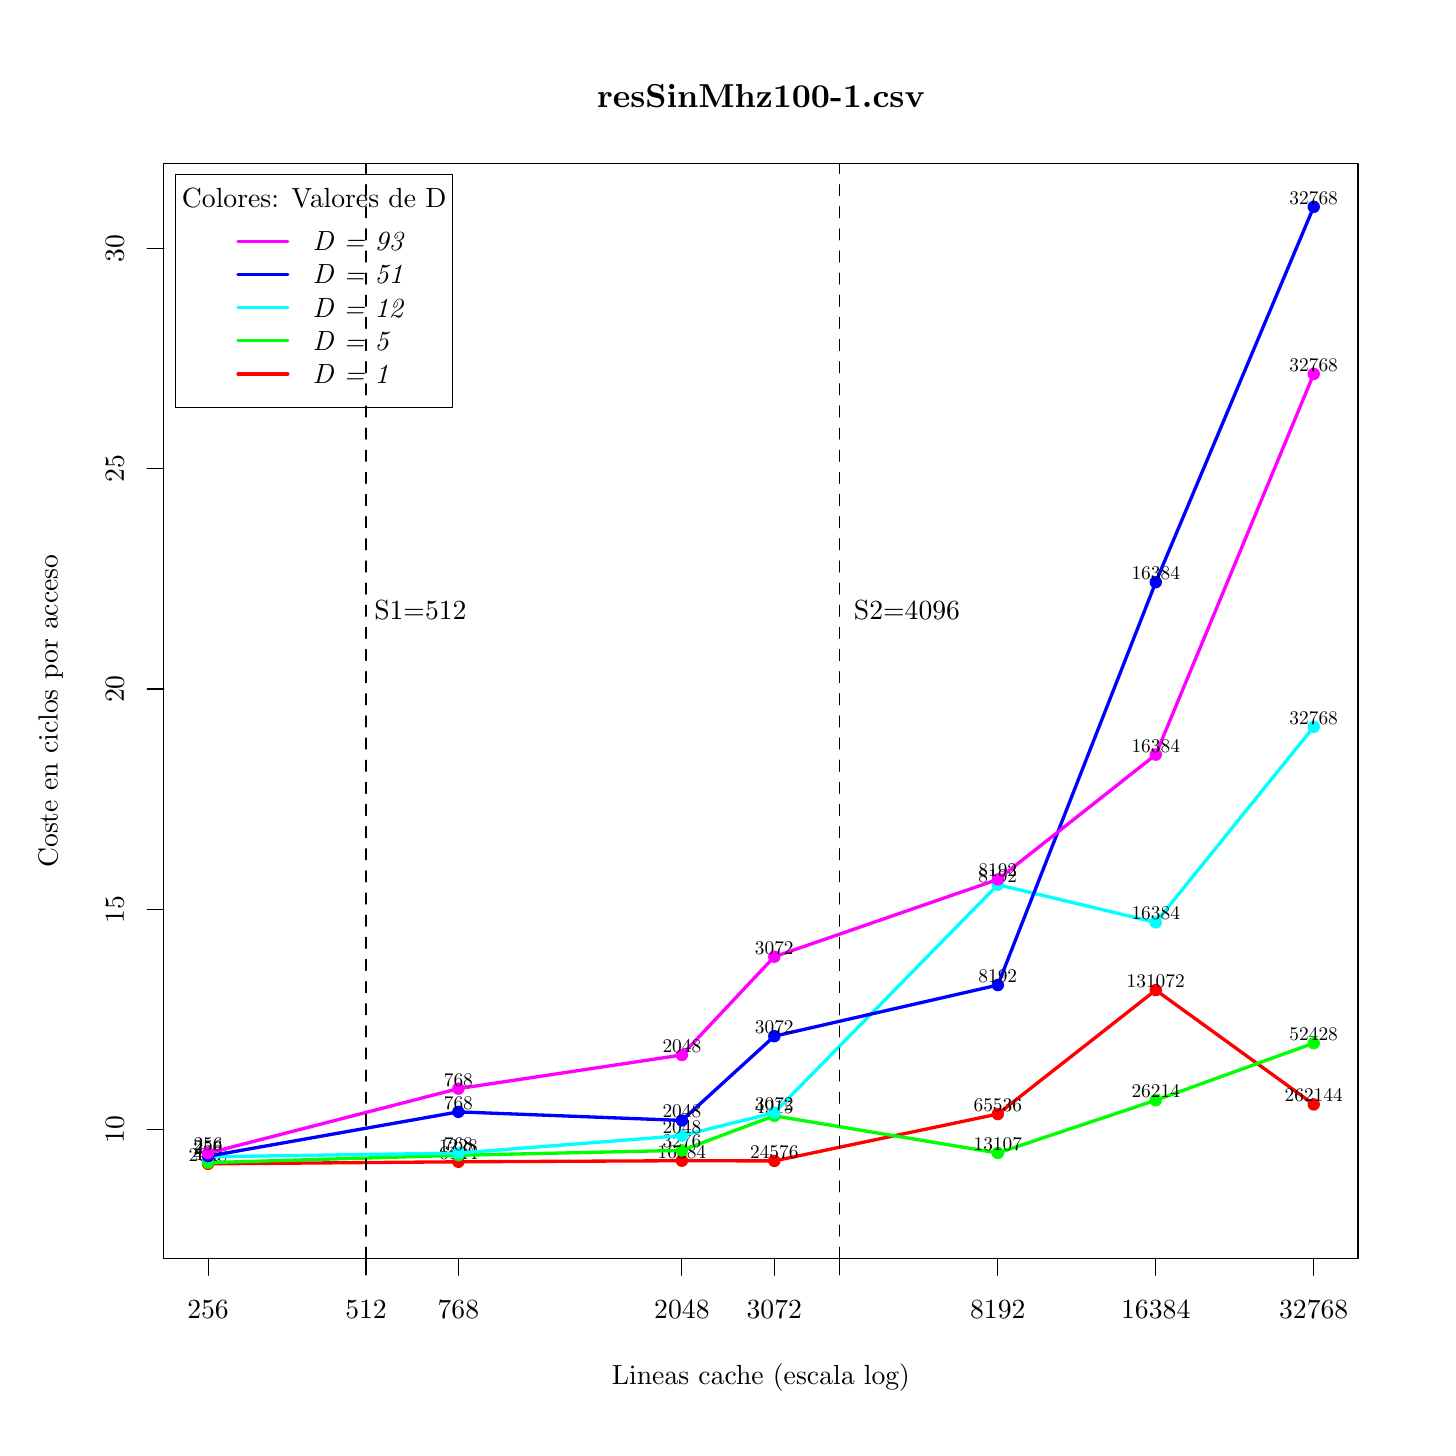
\begin{tikzpicture}[x=1pt,y=1pt]
\definecolor{fillColor}{RGB}{255,255,255}
\path[use as bounding box,fill=fillColor,fill opacity=0.00] (0,0) rectangle (505.89,505.89);
\begin{scope}
\path[clip] ( 49.20, 61.20) rectangle (480.69,456.69);
\definecolor{drawColor}{RGB}{255,255,255}

\path[draw=drawColor,line width= 0.4pt,line join=round,line cap=round] ( 65.18, 95.33) circle (  2.25);

\path[draw=drawColor,line width= 0.4pt,line join=round,line cap=round] (155.64, 96.07) circle (  2.25);

\path[draw=drawColor,line width= 0.4pt,line join=round,line cap=round] (236.41, 96.46) circle (  2.25);

\path[draw=drawColor,line width= 0.4pt,line join=round,line cap=round] (269.79, 96.39) circle (  2.25);

\path[draw=drawColor,line width= 0.4pt,line join=round,line cap=round] (350.56,113.32) circle (  2.25);

\path[draw=drawColor,line width= 0.4pt,line join=round,line cap=round] (407.63,158.11) circle (  2.25);

\path[draw=drawColor,line width= 0.4pt,line join=round,line cap=round] (464.71,116.80) circle (  2.25);

\path[draw=drawColor,line width= 0.4pt,line join=round,line cap=round] ( 65.18, 95.76) circle (  2.25);

\path[draw=drawColor,line width= 0.4pt,line join=round,line cap=round] (155.64, 98.42) circle (  2.25);

\path[draw=drawColor,line width= 0.4pt,line join=round,line cap=round] (236.41,100.21) circle (  2.25);

\path[draw=drawColor,line width= 0.4pt,line join=round,line cap=round] (269.79,112.69) circle (  2.25);

\path[draw=drawColor,line width= 0.4pt,line join=round,line cap=round] (350.56, 99.25) circle (  2.25);

\path[draw=drawColor,line width= 0.4pt,line join=round,line cap=round] (407.63,118.32) circle (  2.25);

\path[draw=drawColor,line width= 0.4pt,line join=round,line cap=round] (464.71,138.95) circle (  2.25);

\path[draw=drawColor,line width= 0.4pt,line join=round,line cap=round] ( 65.18, 97.88) circle (  2.25);

\path[draw=drawColor,line width= 0.4pt,line join=round,line cap=round] (155.64, 99.21) circle (  2.25);

\path[draw=drawColor,line width= 0.4pt,line join=round,line cap=round] (236.41,105.51) circle (  2.25);

\path[draw=drawColor,line width= 0.4pt,line join=round,line cap=round] (269.79,113.82) circle (  2.25);

\path[draw=drawColor,line width= 0.4pt,line join=round,line cap=round] (350.56,196.20) circle (  2.25);

\path[draw=drawColor,line width= 0.4pt,line join=round,line cap=round] (407.63,182.58) circle (  2.25);

\path[draw=drawColor,line width= 0.4pt,line join=round,line cap=round] (464.71,253.23) circle (  2.25);

\path[draw=drawColor,line width= 0.4pt,line join=round,line cap=round] ( 65.18, 98.09) circle (  2.25);

\path[draw=drawColor,line width= 0.4pt,line join=round,line cap=round] (155.64,114.11) circle (  2.25);

\path[draw=drawColor,line width= 0.4pt,line join=round,line cap=round] (236.41,111.02) circle (  2.25);

\path[draw=drawColor,line width= 0.4pt,line join=round,line cap=round] (269.79,141.46) circle (  2.25);

\path[draw=drawColor,line width= 0.4pt,line join=round,line cap=round] (350.56,159.93) circle (  2.25);

\path[draw=drawColor,line width= 0.4pt,line join=round,line cap=round] (407.63,305.51) circle (  2.25);

\path[draw=drawColor,line width= 0.4pt,line join=round,line cap=round] (464.71,441.15) circle (  2.25);

\path[draw=drawColor,line width= 0.4pt,line join=round,line cap=round] ( 65.18, 99.20) circle (  2.25);

\path[draw=drawColor,line width= 0.4pt,line join=round,line cap=round] (155.64,122.51) circle (  2.25);

\path[draw=drawColor,line width= 0.4pt,line join=round,line cap=round] (236.41,134.67) circle (  2.25);

\path[draw=drawColor,line width= 0.4pt,line join=round,line cap=round] (269.79,170.18) circle (  2.25);

\path[draw=drawColor,line width= 0.4pt,line join=round,line cap=round] (350.56,198.10) circle (  2.25);

\path[draw=drawColor,line width= 0.4pt,line join=round,line cap=round] (407.63,243.19) circle (  2.25);

\path[draw=drawColor,line width= 0.4pt,line join=round,line cap=round] (464.71,380.76) circle (  2.25);
\end{scope}
\begin{scope}
\path[clip] (  0.00,  0.00) rectangle (505.89,505.89);
\definecolor{drawColor}{RGB}{0,0,0}

\path[draw=drawColor,line width= 0.4pt,line join=round,line cap=round] ( 49.20,107.69) -- ( 49.20,426.12);

\path[draw=drawColor,line width= 0.4pt,line join=round,line cap=round] ( 49.20,107.69) -- ( 43.20,107.69);

\path[draw=drawColor,line width= 0.4pt,line join=round,line cap=round] ( 49.20,187.30) -- ( 43.20,187.30);

\path[draw=drawColor,line width= 0.4pt,line join=round,line cap=round] ( 49.20,266.91) -- ( 43.20,266.91);

\path[draw=drawColor,line width= 0.4pt,line join=round,line cap=round] ( 49.20,346.51) -- ( 43.20,346.51);

\path[draw=drawColor,line width= 0.4pt,line join=round,line cap=round] ( 49.20,426.12) -- ( 43.20,426.12);

\node[text=drawColor,rotate= 90.00,anchor=base,inner sep=0pt, outer sep=0pt, scale=  1.00] at ( 34.80,107.69) {10};

\node[text=drawColor,rotate= 90.00,anchor=base,inner sep=0pt, outer sep=0pt, scale=  1.00] at ( 34.80,187.30) {15};

\node[text=drawColor,rotate= 90.00,anchor=base,inner sep=0pt, outer sep=0pt, scale=  1.00] at ( 34.80,266.91) {20};

\node[text=drawColor,rotate= 90.00,anchor=base,inner sep=0pt, outer sep=0pt, scale=  1.00] at ( 34.80,346.51) {25};

\node[text=drawColor,rotate= 90.00,anchor=base,inner sep=0pt, outer sep=0pt, scale=  1.00] at ( 34.80,426.12) {30};

\path[draw=drawColor,line width= 0.4pt,line join=round,line cap=round] ( 49.20, 61.20) --
	(480.69, 61.20) --
	(480.69,456.69) --
	( 49.20,456.69) --
	( 49.20, 61.20);
\end{scope}
\begin{scope}
\path[clip] (  0.00,  0.00) rectangle (505.89,505.89);
\definecolor{drawColor}{RGB}{0,0,0}

\node[text=drawColor,anchor=base,inner sep=0pt, outer sep=0pt, scale=  1.20] at (264.94,477.15) {\bfseries resSinMhz100-1.csv};

\node[text=drawColor,anchor=base,inner sep=0pt, outer sep=0pt, scale=  1.00] at (264.94, 15.60) {Lineas cache (escala log)};

\node[text=drawColor,rotate= 90.00,anchor=base,inner sep=0pt, outer sep=0pt, scale=  1.00] at ( 10.80,258.94) {Coste en ciclos por acceso};
\end{scope}
\begin{scope}
\path[clip] (  0.00,  0.00) rectangle (505.89,505.89);
\definecolor{drawColor}{RGB}{0,0,0}

\path[draw=drawColor,line width= 0.4pt,line join=round,line cap=round] ( 65.18, 61.20) -- (464.71, 61.20);

\path[draw=drawColor,line width= 0.4pt,line join=round,line cap=round] ( 65.18, 61.20) -- ( 65.18, 55.20);

\path[draw=drawColor,line width= 0.4pt,line join=round,line cap=round] ( 65.18, 61.20) -- ( 65.18, 55.20);

\path[draw=drawColor,line width= 0.4pt,line join=round,line cap=round] ( 65.18, 61.20) -- ( 65.18, 55.20);

\path[draw=drawColor,line width= 0.4pt,line join=round,line cap=round] ( 65.18, 61.20) -- ( 65.18, 55.20);

\path[draw=drawColor,line width= 0.4pt,line join=round,line cap=round] ( 65.18, 61.20) -- ( 65.18, 55.20);

\path[draw=drawColor,line width= 0.4pt,line join=round,line cap=round] (122.26, 61.20) -- (122.26, 55.20);

\path[draw=drawColor,line width= 0.4pt,line join=round,line cap=round] (155.64, 61.20) -- (155.64, 55.20);

\path[draw=drawColor,line width= 0.4pt,line join=round,line cap=round] (155.64, 61.20) -- (155.64, 55.20);

\path[draw=drawColor,line width= 0.4pt,line join=round,line cap=round] (155.64, 61.20) -- (155.64, 55.20);

\path[draw=drawColor,line width= 0.4pt,line join=round,line cap=round] (155.64, 61.20) -- (155.64, 55.20);

\path[draw=drawColor,line width= 0.4pt,line join=round,line cap=round] (155.64, 61.20) -- (155.64, 55.20);

\path[draw=drawColor,line width= 0.4pt,line join=round,line cap=round] (236.41, 61.20) -- (236.41, 55.20);

\path[draw=drawColor,line width= 0.4pt,line join=round,line cap=round] (236.41, 61.20) -- (236.41, 55.20);

\path[draw=drawColor,line width= 0.4pt,line join=round,line cap=round] (236.41, 61.20) -- (236.41, 55.20);

\path[draw=drawColor,line width= 0.4pt,line join=round,line cap=round] (236.41, 61.20) -- (236.41, 55.20);

\path[draw=drawColor,line width= 0.4pt,line join=round,line cap=round] (236.41, 61.20) -- (236.41, 55.20);

\path[draw=drawColor,line width= 0.4pt,line join=round,line cap=round] (269.79, 61.20) -- (269.79, 55.20);

\path[draw=drawColor,line width= 0.4pt,line join=round,line cap=round] (269.79, 61.20) -- (269.79, 55.20);

\path[draw=drawColor,line width= 0.4pt,line join=round,line cap=round] (269.79, 61.20) -- (269.79, 55.20);

\path[draw=drawColor,line width= 0.4pt,line join=round,line cap=round] (269.79, 61.20) -- (269.79, 55.20);

\path[draw=drawColor,line width= 0.4pt,line join=round,line cap=round] (269.79, 61.20) -- (269.79, 55.20);

\path[draw=drawColor,line width= 0.4pt,line join=round,line cap=round] (293.48, 61.20) -- (293.48, 55.20);

\path[draw=drawColor,line width= 0.4pt,line join=round,line cap=round] (350.56, 61.20) -- (350.56, 55.20);

\path[draw=drawColor,line width= 0.4pt,line join=round,line cap=round] (350.56, 61.20) -- (350.56, 55.20);

\path[draw=drawColor,line width= 0.4pt,line join=round,line cap=round] (350.56, 61.20) -- (350.56, 55.20);

\path[draw=drawColor,line width= 0.4pt,line join=round,line cap=round] (350.56, 61.20) -- (350.56, 55.20);

\path[draw=drawColor,line width= 0.4pt,line join=round,line cap=round] (350.56, 61.20) -- (350.56, 55.20);

\path[draw=drawColor,line width= 0.4pt,line join=round,line cap=round] (407.63, 61.20) -- (407.63, 55.20);

\path[draw=drawColor,line width= 0.4pt,line join=round,line cap=round] (407.63, 61.20) -- (407.63, 55.20);

\path[draw=drawColor,line width= 0.4pt,line join=round,line cap=round] (407.63, 61.20) -- (407.63, 55.20);

\path[draw=drawColor,line width= 0.4pt,line join=round,line cap=round] (407.63, 61.20) -- (407.63, 55.20);

\path[draw=drawColor,line width= 0.4pt,line join=round,line cap=round] (407.63, 61.20) -- (407.63, 55.20);

\path[draw=drawColor,line width= 0.4pt,line join=round,line cap=round] (464.71, 61.20) -- (464.71, 55.20);

\path[draw=drawColor,line width= 0.4pt,line join=round,line cap=round] (464.71, 61.20) -- (464.71, 55.20);

\path[draw=drawColor,line width= 0.4pt,line join=round,line cap=round] (464.71, 61.20) -- (464.71, 55.20);

\path[draw=drawColor,line width= 0.4pt,line join=round,line cap=round] (464.71, 61.20) -- (464.71, 55.20);

\path[draw=drawColor,line width= 0.4pt,line join=round,line cap=round] (464.71, 61.20) -- (464.71, 55.20);

\node[text=drawColor,anchor=base,inner sep=0pt, outer sep=0pt, scale=  1.00] at ( 65.18, 39.60) {256};

\node[text=drawColor,anchor=base,inner sep=0pt, outer sep=0pt, scale=  1.00] at (122.26, 39.60) {512};

\node[text=drawColor,anchor=base,inner sep=0pt, outer sep=0pt, scale=  1.00] at (155.64, 39.60) {768};

\node[text=drawColor,anchor=base,inner sep=0pt, outer sep=0pt, scale=  1.00] at (236.41, 39.60) {2048};

\node[text=drawColor,anchor=base,inner sep=0pt, outer sep=0pt, scale=  1.00] at (269.79, 39.60) {3072};

\node[text=drawColor,anchor=base,inner sep=0pt, outer sep=0pt, scale=  1.00] at (350.56, 39.60) {8192};

\node[text=drawColor,anchor=base,inner sep=0pt, outer sep=0pt, scale=  1.00] at (407.63, 39.60) {16384};

\node[text=drawColor,anchor=base,inner sep=0pt, outer sep=0pt, scale=  1.00] at (464.71, 39.60) {32768};
\end{scope}
\begin{scope}
\path[clip] ( 49.20, 61.20) rectangle (480.69,456.69);
\definecolor{fillColor}{RGB}{255,0,0}

\path[fill=fillColor] ( 65.18, 95.33) circle (  2.25);

\path[fill=fillColor] (155.64, 96.07) circle (  2.25);

\path[fill=fillColor] (236.41, 96.46) circle (  2.25);

\path[fill=fillColor] (269.79, 96.39) circle (  2.25);

\path[fill=fillColor] (350.56,113.32) circle (  2.25);

\path[fill=fillColor] (407.63,158.11) circle (  2.25);

\path[fill=fillColor] (464.71,116.80) circle (  2.25);
\definecolor{drawColor}{RGB}{255,0,0}

\path[draw=drawColor,line width= 1.2pt,line join=round,line cap=round] ( 65.18, 95.33) --
	(155.64, 96.07) --
	(236.41, 96.46) --
	(269.79, 96.39) --
	(350.56,113.32) --
	(407.63,158.11) --
	(464.71,116.80);
\definecolor{drawColor}{RGB}{0,0,0}

\node[text=drawColor,anchor=base,inner sep=0pt, outer sep=0pt, scale=  0.70] at ( 65.18, 96.27) {2048};

\node[text=drawColor,anchor=base,inner sep=0pt, outer sep=0pt, scale=  0.70] at (155.64, 97.01) {6144};

\node[text=drawColor,anchor=base,inner sep=0pt, outer sep=0pt, scale=  0.70] at (236.41, 97.40) {16384};

\node[text=drawColor,anchor=base,inner sep=0pt, outer sep=0pt, scale=  0.70] at (269.79, 97.33) {24576};

\node[text=drawColor,anchor=base,inner sep=0pt, outer sep=0pt, scale=  0.70] at (350.56,114.26) {65536};

\node[text=drawColor,anchor=base,inner sep=0pt, outer sep=0pt, scale=  0.70] at (407.63,159.05) {131072};

\node[text=drawColor,anchor=base,inner sep=0pt, outer sep=0pt, scale=  0.70] at (464.71,117.74) {262144};
\definecolor{fillColor}{RGB}{0,255,0}

\path[fill=fillColor] ( 65.18, 95.76) circle (  2.25);

\path[fill=fillColor] (155.64, 98.42) circle (  2.25);

\path[fill=fillColor] (236.41,100.21) circle (  2.25);

\path[fill=fillColor] (269.79,112.69) circle (  2.25);

\path[fill=fillColor] (350.56, 99.25) circle (  2.25);

\path[fill=fillColor] (407.63,118.32) circle (  2.25);

\path[fill=fillColor] (464.71,138.95) circle (  2.25);
\definecolor{drawColor}{RGB}{0,255,0}

\path[draw=drawColor,line width= 1.2pt,line join=round,line cap=round] ( 65.18, 95.76) --
	(155.64, 98.42) --
	(236.41,100.21) --
	(269.79,112.69) --
	(350.56, 99.25) --
	(407.63,118.32) --
	(464.71,138.95);
\definecolor{drawColor}{RGB}{0,0,0}

\node[text=drawColor,anchor=base,inner sep=0pt, outer sep=0pt, scale=  0.70] at ( 65.18, 96.70) {409};

\node[text=drawColor,anchor=base,inner sep=0pt, outer sep=0pt, scale=  0.70] at (155.64, 99.36) {1228};

\node[text=drawColor,anchor=base,inner sep=0pt, outer sep=0pt, scale=  0.70] at (236.41,101.15) {3276};

\node[text=drawColor,anchor=base,inner sep=0pt, outer sep=0pt, scale=  0.70] at (269.79,113.63) {4915};

\node[text=drawColor,anchor=base,inner sep=0pt, outer sep=0pt, scale=  0.70] at (350.56,100.19) {13107};

\node[text=drawColor,anchor=base,inner sep=0pt, outer sep=0pt, scale=  0.70] at (407.63,119.26) {26214};

\node[text=drawColor,anchor=base,inner sep=0pt, outer sep=0pt, scale=  0.70] at (464.71,139.89) {52428};
\definecolor{fillColor}{RGB}{0,255,255}

\path[fill=fillColor] ( 65.18, 97.88) circle (  2.25);

\path[fill=fillColor] (155.64, 99.21) circle (  2.25);

\path[fill=fillColor] (236.41,105.51) circle (  2.25);

\path[fill=fillColor] (269.79,113.82) circle (  2.25);

\path[fill=fillColor] (350.56,196.20) circle (  2.25);

\path[fill=fillColor] (407.63,182.58) circle (  2.25);

\path[fill=fillColor] (464.71,253.23) circle (  2.25);
\definecolor{drawColor}{RGB}{0,255,255}

\path[draw=drawColor,line width= 1.2pt,line join=round,line cap=round] ( 65.18, 97.88) --
	(155.64, 99.21) --
	(236.41,105.51) --
	(269.79,113.82) --
	(350.56,196.20) --
	(407.63,182.58) --
	(464.71,253.23);
\definecolor{drawColor}{RGB}{0,0,0}

\node[text=drawColor,anchor=base,inner sep=0pt, outer sep=0pt, scale=  0.70] at ( 65.18, 98.82) {256};

\node[text=drawColor,anchor=base,inner sep=0pt, outer sep=0pt, scale=  0.70] at (155.64,100.15) {768};

\node[text=drawColor,anchor=base,inner sep=0pt, outer sep=0pt, scale=  0.70] at (236.41,106.45) {2048};

\node[text=drawColor,anchor=base,inner sep=0pt, outer sep=0pt, scale=  0.70] at (269.79,114.76) {3072};

\node[text=drawColor,anchor=base,inner sep=0pt, outer sep=0pt, scale=  0.70] at (350.56,197.14) {8192};

\node[text=drawColor,anchor=base,inner sep=0pt, outer sep=0pt, scale=  0.70] at (407.63,183.52) {16384};

\node[text=drawColor,anchor=base,inner sep=0pt, outer sep=0pt, scale=  0.70] at (464.71,254.17) {32768};
\definecolor{fillColor}{RGB}{0,0,255}

\path[fill=fillColor] ( 65.18, 98.09) circle (  2.25);

\path[fill=fillColor] (155.64,114.11) circle (  2.25);

\path[fill=fillColor] (236.41,111.02) circle (  2.25);

\path[fill=fillColor] (269.79,141.46) circle (  2.25);

\path[fill=fillColor] (350.56,159.93) circle (  2.25);

\path[fill=fillColor] (407.63,305.51) circle (  2.25);

\path[fill=fillColor] (464.71,441.15) circle (  2.25);
\definecolor{drawColor}{RGB}{0,0,255}

\path[draw=drawColor,line width= 1.2pt,line join=round,line cap=round] ( 65.18, 98.09) --
	(155.64,114.11) --
	(236.41,111.02) --
	(269.79,141.46) --
	(350.56,159.93) --
	(407.63,305.51) --
	(464.71,441.15);
\definecolor{drawColor}{RGB}{0,0,0}

\node[text=drawColor,anchor=base,inner sep=0pt, outer sep=0pt, scale=  0.70] at ( 65.18, 99.03) {256};

\node[text=drawColor,anchor=base,inner sep=0pt, outer sep=0pt, scale=  0.70] at (155.64,115.05) {768};

\node[text=drawColor,anchor=base,inner sep=0pt, outer sep=0pt, scale=  0.70] at (236.41,111.96) {2048};

\node[text=drawColor,anchor=base,inner sep=0pt, outer sep=0pt, scale=  0.70] at (269.79,142.40) {3072};

\node[text=drawColor,anchor=base,inner sep=0pt, outer sep=0pt, scale=  0.70] at (350.56,160.87) {8192};

\node[text=drawColor,anchor=base,inner sep=0pt, outer sep=0pt, scale=  0.70] at (407.63,306.45) {16384};

\node[text=drawColor,anchor=base,inner sep=0pt, outer sep=0pt, scale=  0.70] at (464.71,442.08) {32768};
\definecolor{fillColor}{RGB}{255,0,255}

\path[fill=fillColor] ( 65.18, 99.20) circle (  2.25);

\path[fill=fillColor] (155.64,122.51) circle (  2.25);

\path[fill=fillColor] (236.41,134.67) circle (  2.25);

\path[fill=fillColor] (269.79,170.18) circle (  2.25);

\path[fill=fillColor] (350.56,198.10) circle (  2.25);

\path[fill=fillColor] (407.63,243.19) circle (  2.25);

\path[fill=fillColor] (464.71,380.76) circle (  2.25);
\definecolor{drawColor}{RGB}{255,0,255}

\path[draw=drawColor,line width= 1.2pt,line join=round,line cap=round] ( 65.18, 99.20) --
	(155.64,122.51) --
	(236.41,134.67) --
	(269.79,170.18) --
	(350.56,198.10) --
	(407.63,243.19) --
	(464.71,380.76);
\definecolor{drawColor}{RGB}{0,0,0}

\node[text=drawColor,anchor=base,inner sep=0pt, outer sep=0pt, scale=  0.70] at ( 65.18,100.14) {256};

\node[text=drawColor,anchor=base,inner sep=0pt, outer sep=0pt, scale=  0.70] at (155.64,123.45) {768};

\node[text=drawColor,anchor=base,inner sep=0pt, outer sep=0pt, scale=  0.70] at (236.41,135.61) {2048};

\node[text=drawColor,anchor=base,inner sep=0pt, outer sep=0pt, scale=  0.70] at (269.79,171.12) {3072};

\node[text=drawColor,anchor=base,inner sep=0pt, outer sep=0pt, scale=  0.70] at (350.56,199.04) {8192};

\node[text=drawColor,anchor=base,inner sep=0pt, outer sep=0pt, scale=  0.70] at (407.63,244.13) {16384};

\node[text=drawColor,anchor=base,inner sep=0pt, outer sep=0pt, scale=  0.70] at (464.71,381.70) {32768};

\node[text=drawColor,anchor=base,inner sep=0pt, outer sep=0pt, scale=  1.00] at (141.91,292.12) {S1=512};

\node[text=drawColor,anchor=base,inner sep=0pt, outer sep=0pt, scale=  1.00] at (317.75,292.12) {S2=4096};

\path[draw=drawColor,line width= 0.4pt,dash pattern=on 4pt off 4pt ,line join=round,line cap=round] (122.26, 61.20) -- (122.26,456.69);

\path[draw=drawColor,line width= 0.4pt,dash pattern=on 4pt off 4pt ,line join=round,line cap=round] (293.48, 61.20) -- (293.48,456.69);

\path[draw=drawColor,line width= 0.4pt,line join=round,line cap=round] ( 53.51,452.74) rectangle (153.57,368.74);
\definecolor{drawColor}{RGB}{255,0,255}

\path[draw=drawColor,line width= 1.2pt,line join=round,line cap=round] ( 76.00,428.74) -- ( 94.00,428.74);
\definecolor{drawColor}{RGB}{0,0,255}

\path[draw=drawColor,line width= 1.2pt,line join=round,line cap=round] ( 76.00,416.74) -- ( 94.00,416.74);
\definecolor{drawColor}{RGB}{0,255,255}

\path[draw=drawColor,line width= 1.2pt,line join=round,line cap=round] ( 76.00,404.74) -- ( 94.00,404.74);
\definecolor{drawColor}{RGB}{0,255,0}

\path[draw=drawColor,line width= 1.2pt,line join=round,line cap=round] ( 76.00,392.74) -- ( 94.00,392.74);
\definecolor{drawColor}{RGB}{255,0,0}

\path[draw=drawColor,line width= 1.2pt,line join=round,line cap=round] ( 76.00,380.74) -- ( 94.00,380.74);
\definecolor{drawColor}{RGB}{0,0,0}

\node[text=drawColor,anchor=base,inner sep=0pt, outer sep=0pt, scale=  1.00] at (103.54,440.74) {Colores: Valores de D};

\node[text=drawColor,anchor=base west,inner sep=0pt, outer sep=0pt, scale=  1.00] at (103.00,425.29) {\itshape D = 93};

\node[text=drawColor,anchor=base west,inner sep=0pt, outer sep=0pt, scale=  1.00] at (103.00,413.29) {\itshape D = 51};

\node[text=drawColor,anchor=base west,inner sep=0pt, outer sep=0pt, scale=  1.00] at (103.00,401.29) {\itshape D = 12};

\node[text=drawColor,anchor=base west,inner sep=0pt, outer sep=0pt, scale=  1.00] at (103.00,389.29) {\itshape D = 5};

\node[text=drawColor,anchor=base west,inner sep=0pt, outer sep=0pt, scale=  1.00] at (103.00,377.29) {\itshape D = 1};
\end{scope}
\end{tikzpicture}
